\section{eo\-UF$<$ A1, R $>$ Class Template Reference}
\label{classeo_u_f}\index{eoUF@{eoUF}}
Basic Unary Functor.  


{\tt \#include $<$eo\-Functor.h$>$}

Inheritance diagram for eo\-UF$<$ A1, R $>$::\begin{figure}[H]
\begin{center}
\leavevmode
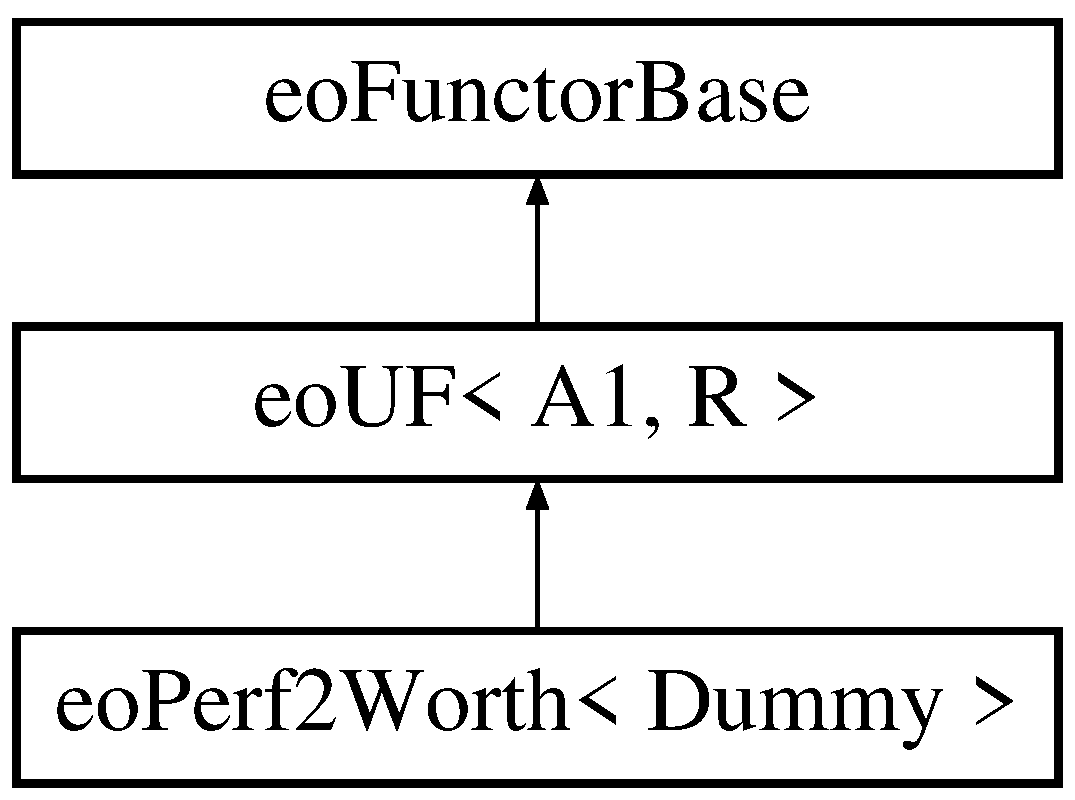
\includegraphics[height=3cm]{classeo_u_f}
\end{center}
\end{figure}
\subsection*{Public Member Functions}
\begin{CompactItemize}
\item 
virtual {\bf $\sim$eo\-UF} ()\label{classeo_u_f_a0}

\begin{CompactList}\small\item\em virtual dtor here so there is no need to define it in derived classes \item\end{CompactList}\item 
virtual R {\bf operator()} (A1)=0\label{classeo_u_f_a1}

\begin{CompactList}\small\item\em The pure virtual function that needs to be implemented by the subclass. \item\end{CompactList}\end{CompactItemize}
\subsection*{Static Public Member Functions}
\begin{CompactItemize}
\item 
{\bf eo\-Functor\-Base::unary\_\-function\_\-tag} {\bf functor\_\-category} ()\label{classeo_u_f_e0}

\begin{CompactList}\small\item\em tag to identify a procedure in compile time function selection functor\_\-category \item\end{CompactList}\end{CompactItemize}


\subsection{Detailed Description}
\subsubsection*{template$<$class A1, class R$>$ class eo\-UF$<$ A1, R $>$}

Basic Unary Functor. 

Derive from this class when defining any unary function. First template argument is the first\_\-argument\_\-type, second result\_\-type. Argument and result types can be any type including void for result\_\-type 



Definition at line 108 of file eo\-Functor.h.

The documentation for this class was generated from the following file:\begin{CompactItemize}
\item 
eo\-Functor.h\end{CompactItemize}
